\documentclass[a4paper,14pt]{extarticle}

\usepackage{indentfirst}
\usepackage[utf8]{inputenc}
\usepackage[T1]{fontenc}
\usepackage[utf8]{vietnam}
\usepackage{float}
\usepackage{hyperref}

\usepackage{ifxetex,ifluatex}
\usepackage{etoolbox}
\usepackage[svgnames]{xcolor}

\usepackage{tikz}
\usepackage{framed}

\usepackage{enumitem}
\setitemize{itemsep=1pt}
\setlist{nolistsep}

\usepackage{caption}

\newcommand*\quotefont{}
\newcommand*\quotesize{60}
\newcommand*{\openquote}
	{\tikz[remember picture,overlay,xshift=-4ex,yshift=-2.5ex]
	\node (OQ) {\quotefont\fontsize{\quotesize}{\quotesize}\selectfont``};\kern0pt}

\newcommand*{\closequote}[1]
	{\tikz[remember picture,overlay,xshift=4ex,yshift={#1}]
	\node (CQ) {\quotefont\fontsize{\quotesize}{\quotesize}\selectfont''};}

\colorlet{shadecolor}{Azure}

\newcommand*\shadedauthorformat{\emph}

\newcommand*\authoralign[1]{%
	\if#1l
		\def\authorfill{}\def\quotefill{\hfill}
	\else
		\if#1r
			\def\authorfill{\hfill}\def\quotefill{}
		\else
			\if#1c
				\gdef\authorfill{\hfill}\def\quotefill{\hfill}
			\else\typeout{Invalid option}
			\fi
		\fi
	\fi}

\newenvironment{shadequote}[2][l]%
{\authoralign{#1}
\ifblank{#2}
	{\def\shadequoteauthor{}\def\yshift{-2ex}\def\quotefill{\hfill}}
	{\def\shadequoteauthor{\par\authorfill\shadedauthorformat{#2}}\def\yshift{2ex}}
\begin{snugshade}\begin{quote}\openquote}
{\shadequoteauthor\quotefill\closequote{\yshift}\end{quote}\end{snugshade}}

\usepackage{geometry}
\geometry{
a4paper,
% total={170mm,257mm},
left=30mm,
right=20mm,
top=20mm,
bottom=20mm,
}

% ============ Document starts here ==============

\title{\textbf{Nhận diện một số sâu bệnh\\thường gặp trên cây cà phê\\qua hình thái của lá}}
\author{Nguyễn Quang Trường\\12 Toán - Trường THPT Chuyên Nguyễn Tất Thành}
\date{Kon Tum, ngày 15 tháng 12 năn 2021}

\begin{document}

\tableofcontents

\pagebreak

\section{Lý do chọn đề tài}
Kon Tum là một tỉnh thuộc khu vực Tây Nguyên, nổi tiếng với những loài cây công nghiệp lâu năm. Trong đó, cà phê có vai trò quan trọng đối với người dân nơi đây, đặc biệt là với đồng bào dân tộc thiểu số, giúp xóa đói, giảm nghèo, mang lại nguồn thu nhập lớn cho nhân dân tỉnh nhà.

\begin{shadequote}[l]{- Bộ Nông nghiệp và Phát triển Nông thôn (2017)}
	...Cà phê là sản phẩm chiếm tỷ trọng lớn trong xã hội và kim ngạch xuất khẩu hằng năm của tỉnh Kon Tum, tạo ra nguồn thu nhập chính cho người dân các huyện sinh sống trên địa bàn có lợi thế phát triển cà phê, đặc biệt là vùng đồng bào dân tộc thiểu số trồng cà phê chè tại các xã vùng Đông Trường Sơn...
\end{shadequote}

Tuy nhiên, hằng năm, sâu bệnh trên cây cà phê đã gây thiệt hại nặng nề cho bà con và các doanh nghiệp sản xuất, chế biến cà phê bản địa.

Vì vậy, tác giả đã nghiên cứu và phát triển dự án: \textbf{Nhận diện một số sâu bệnh thường gặp trên cây cà phê qua hình thái của lá}. Đây là một hệ thống nhận diện thông minh, tương đối chính xác, nhằm giúp nhân dân, nhất là đồng bào dân tộc thiểu số nhận diện một số sâu bệnh thường gặp trên cây cà phê dễ dàng, thuận tiện để có các biện pháp phòng trừ sâu bệnh hiệu quả, góp phần cải thiện ngành trồng trọt cây cà phê tại tỉnh Kon Tum.

\section{Tìm hiểu vấn đề}

	\subsection{Câu hỏi nghiên cứu}
	Trước khi nghiên cứu, tác giả đưa ra một số câu hỏi nghiên cứu:
	\begin{itemize}
		\item Hiện tại, có những phương pháp nào để chẩn đoán sâu bệnh trên
		cây cà phê?
		\item Nhận dạng các đặc điểm của sâu bệnh bằng mắt thường như thế
		nào? Làm thế nào để máy có thể nhận dạng tương tự?
	\end{itemize}

		\subsubsection{Một số phương pháp hiện tại}
		Theo tìm hiểu của tác giả, hiện nay có hai phương pháp chính để chẩn đoán sâu bệnh.
		
		Phương pháp đầu tiên: chẩn đoán thông qua đặc điểm hình thái trên lá. Ưu điểm là nhanh chóng, thuận tiện, chi phí thấp... Tuy nhiên, nhược điểm rõ ràng nhất là khó phát hiện được các sâu bệnh phức tạp, ít thể hiện trên hình thái mà phải phân tích chuyên sâu.
		
		Phương pháp thứ hai: phân tích cấu trúc lá trong phòng thí nghiệm. Phương pháp này cho độ chính xác cao hơn, xác định được những sâu bệnh phức tạp hơn mà không thể quan sát bằng mắt thường. Nhưng việc nghiên cứu trong phòng thí nghiệm đòi hỏi nhiều thời gian, công sức để phân tích, chi phí cho cơ sở vật chất...
		
		Với mong muốn xây dựng một giải pháp nhanh chóng và thuận tiện, phương pháp nghiên cứu thông qua đặc điểm hình thái là phương pháp được lựa chọn làm cơ sở cho việc xây dựng giải pháp.

		\subsubsection{Mục tiêu dự án}
		Dự án nghiên cứu nhằm:
		\begin{itemize}
			\item Xây dựng một mô hình giúp nhân dân, đặc biệt là đồng bào dân tộc thiểu số (đa số có trình độ dân trí thấp, chưa biết ứng dụng khoa học kĩ thuật vào canh tác) nhận diện các loại sâu bệnh trên cây cà phê qua hình ảnh với độ chính xác cao;
			\item Ứng dụng mô hình vào thực tiễn tại địa phương, giúp giảm thiểu thiệt hại do sâu bệnh gây ra, góp phần phát triển kinh tế - xã hội trên địa bàn, giúp đồng bào dân tộc thiểu số vươn lên thoát nghèo, làm giàu trên chính quê hương của mình.
		\end{itemize}
			
	\subsection{Ý nghĩa của dự án}
		\subsubsection{Ý nghĩa khoa học}
		Đề tài nghiên cứu phương pháp nhận diện qua hình ảnh, tuy phổ biến trên những đối tượng khác nhưng lại ít được quan tâm trên cây cà phê. Vì vậy, tác giả mong muốn đề tài này sẽ mở rộng nghiên cứu nhận diện hình ảnh trên cây cà phê trong tương lai.

		\subsubsection{Ý nghĩa xã hội}
		Đối tượng nghiên cứu của dự án là cây cà phê, một trong những cây công nghiệp quan trọng ở tỉnh Kon Tum. Do đó, thông qua việc nghiên cứu dự án, tác giả muốn giúp nhân dân, đặc biệt là đồng bào dân tộc thiểu số dễ dàng nhận diện một số sâu bệnh cơ bản để có cách phòng trừ hiệu quả, góp phần xóa đói, giảm nghèo, phát triển kinh tế - xã hội trên địa bàn.

\section{Hệ thống}
	\subsection{Dữ liệu}
	Dữ liệu được kết hợp thu thập từ thực địa, và từ các tập dữ liệu khác trên mạng [4]. Dữ liệu từ thực địa được thu thập tại huyện Đăk Hà (huyện nổi tiếng về sản xuất cà phê trên địa bàn tỉnh Kon Tum) và xã Ia Chim (xã trồng nhiều cây cà phê của thành phố Kon Tum). Ảnh được thu thập từ nhiều thiết bị khác nhau (Samsung Galaxy A02, ASUS Zenfone 2, Xiaomi Redmi 5A, Xiaomi S2, Galaxy S8, và iPhone 6S). Mẫu vật được đặt trên nền trắng, dưới điều kiện kiểm soát một phần.

	Sau một thời gian nghiên cứu và tìm hiểu, một bộ dữ liệu gồm 1747 bức ảnh chụp các lá cà phê (bao gồm lá bình thường và lá sâu bệnh) đã được thu thập.

	\begin{figure}[H]
		\centering
		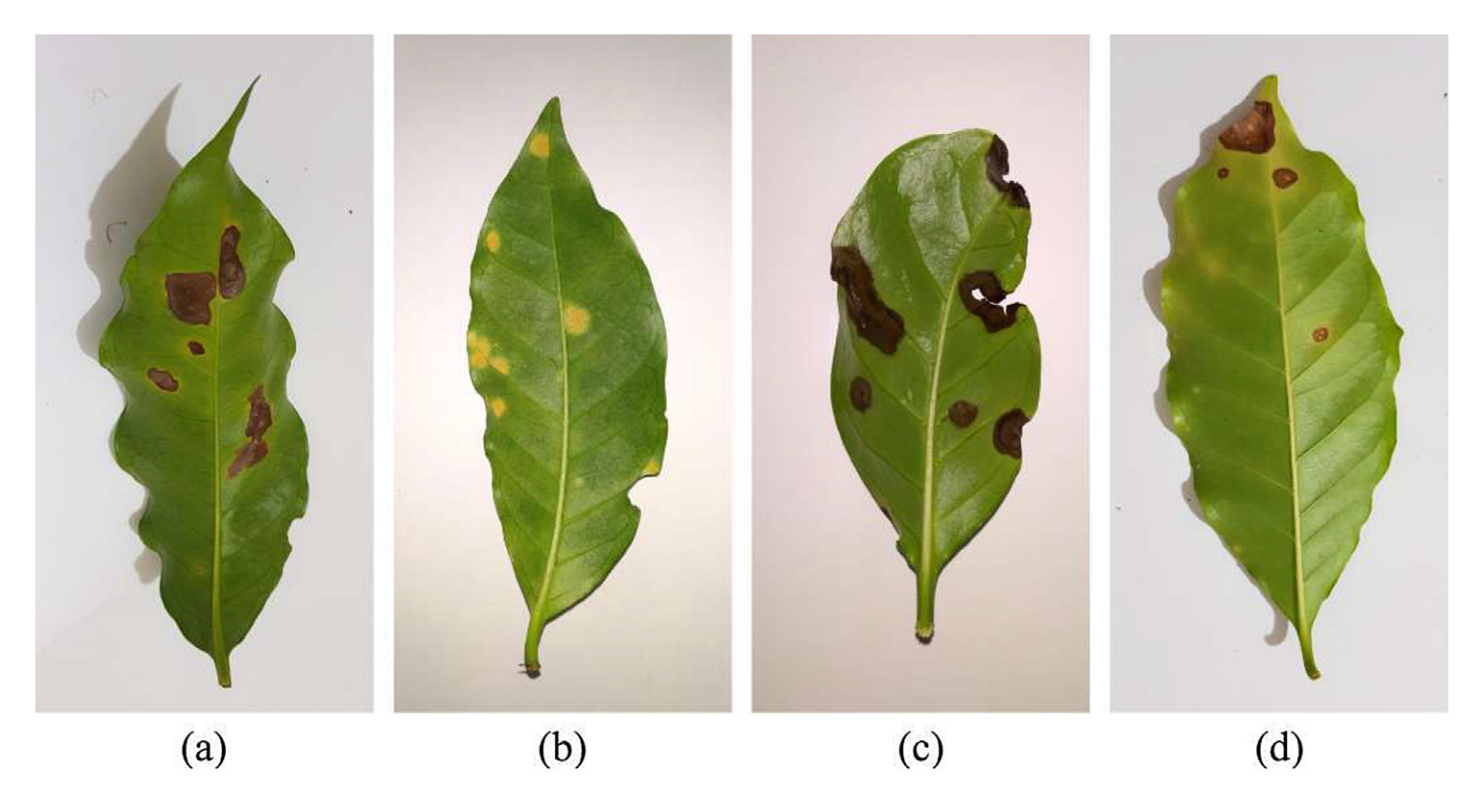
\includegraphics[scale=0.35]{images/image1}
		\caption{sâu vẽ bùa (a), gỉ sắt (b), đốm nâu (c), đốm mắt cua (d)}
	\end{figure}

	Tuy nhiên, mỗi bức ảnh có kích thước rất lớn, gây khó khăn trong quá trình xử lý về sau. Do đó, thay vì giữ nguyên bản, những vùng có sâu bệnh sẽ được cắt ra. Những vùng hoàn toàn bình thường trên lá cũng sẽ được cắt, nhằm mục đích đối chiếu với các vùng sâu bệnh. Sau tiền xử lý, thu được 2722 bức ảnh cắt xung quanh vùng có sâu bệnh và không có sâu bệnh trên lá.
	
	\begin{figure}[H]
		\centering
		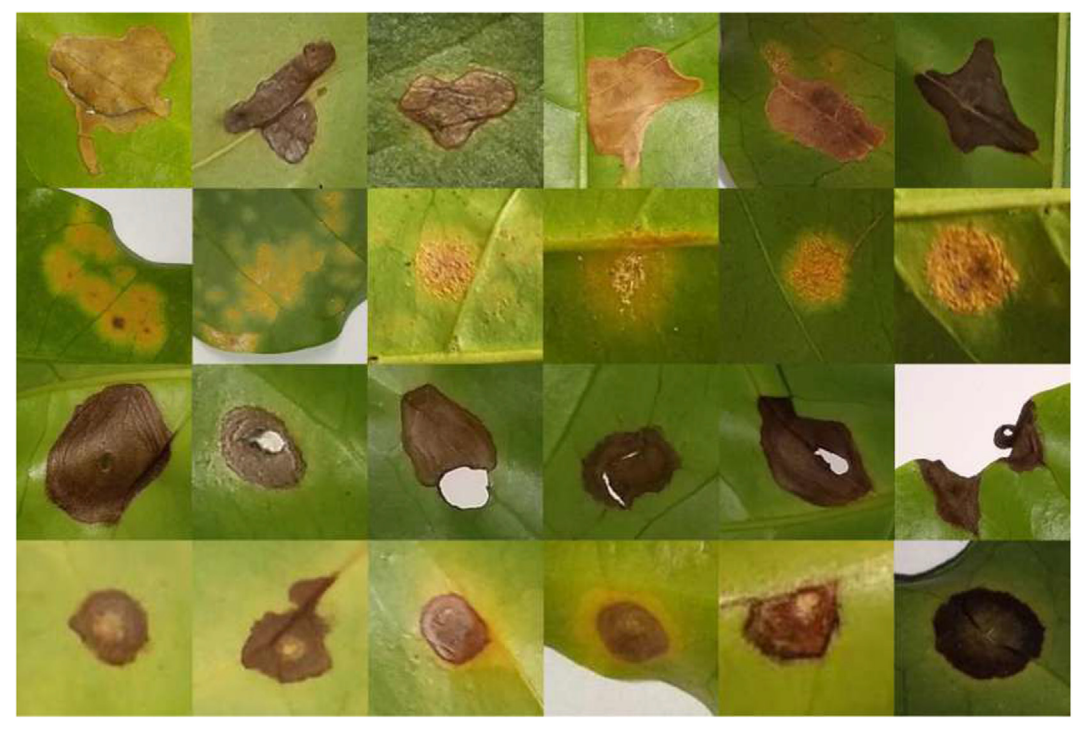
\includegraphics[scale=0.4]{images/image3}
		\caption{Các vùng được cắt sau tiền xử lý}
	\end{figure}

	\begin{table}[H]
		\centering
		\begin{tabular}{|c|c|}
		\hline
		Sâu bệnh        & Số lượng ảnh \\ \hline
		Bình thường & 256          \\
		Sâu vẽ bùa  & 593          \\
		Gỉ sắt      & 991          \\
		Đốm nâu     & 504          \\
		Đốm mắt cua & 378          \\ \hline
		Tổng        & 2722         \\ \hline
		\end{tabular}

		\caption{Thống kê dữ liệu sau tiền xử lý}
	\end{table}

	Tập dữ liệu được chia ra thành 3 tập con riêng biệt, theo tỉ lệ 70-15-15: training set, validation set và test set. Trên thực tế, để rèn luyện cho một mô hình phức tạp, số lượng ảnh thu thập được như trên vẫn chưa đảm bảo, dễ dẫn đến tình trạng overfitting\footnote{Hiện tượng mô hình được luyện quá khớp với bộ dữ liệu sẵn có, dẫn đến mất tính tổng quát và sai lệch khi dự đoán với đầu vào thực tế.}.

	Một kĩ thuật phổ biến để khắc phục vấn đề này là Data Augmentation. Kĩ thuật này lấy những dữ liệu có sẵn trong tập, chỉnh sửa để tạo ra những dữ liệu mới mà không làm mất đi tính chất tổng quát của ảnh.

	\begin{figure}[H]
		\centering
		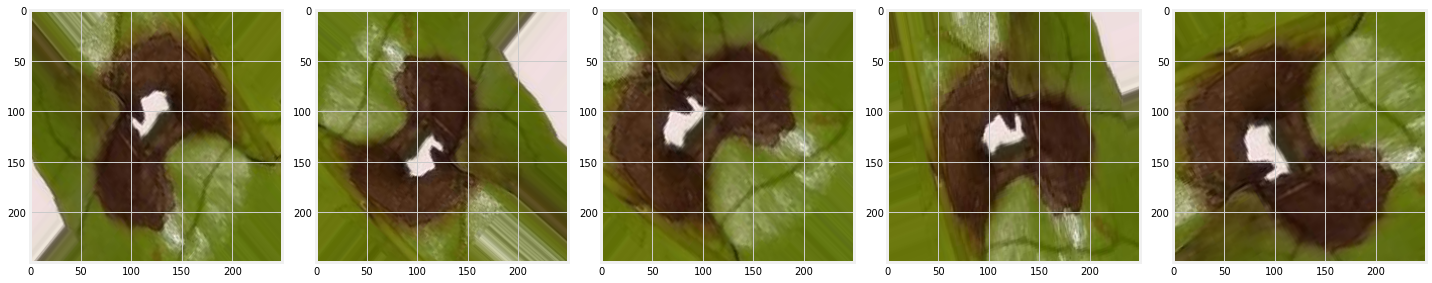
\includegraphics[scale=0.25]{images/image2}
		\caption{Ảnh được chỉnh sửa trong bước Data Augmentation}
	\end{figure}

	\subsection{Mô hình}
	\begin{figure}[H]
		\centering
		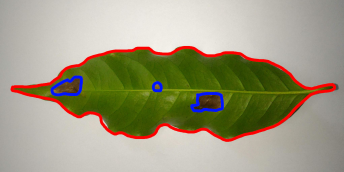
\includegraphics[scale=1]{images/image11}
		\caption{Các khu vực khác nhau của lá}
	\end{figure}

	Một người bình thường sẽ phân tích theo trình tự sau:

	\begin{itemize}
		\item Khu vực bên trong đường màu đỏ là lá. Khu vực bên ngoài
		đường màu đỏ không phải là lá, nên không cần quan tâm;
		\item Khu vực bên trong những đường màu xanh là các vị trí sâu
		bệnh, chỉ cần phân tích đặc điểm của những khu vực này;
		\item Nếu không có khu vực màu xanh nào: lá khỏe mạnh.
	\end{itemize}

	\null

	Sau khi khoanh vùng được vị trí cần quan tâm, con người vận dụng kiến thức (từ kinh nghiệm thực tiễn, từ quá trình học tập...) để kết luận về sâu bệnh.

	Bằng việc xây dựng một mạng lưới mô phỏng hoạt động của các nơ-ron thần kinh trong não bộ con người, một chiếc máy cũng có thể tự học và dự đoán được các loại sâu bệnh khác nhau. Đây chính là nền tảng của Deep Learning, một nhánh con của Trí tuệ Nhân tạo.

	\begin{figure}[H]
		\centering
		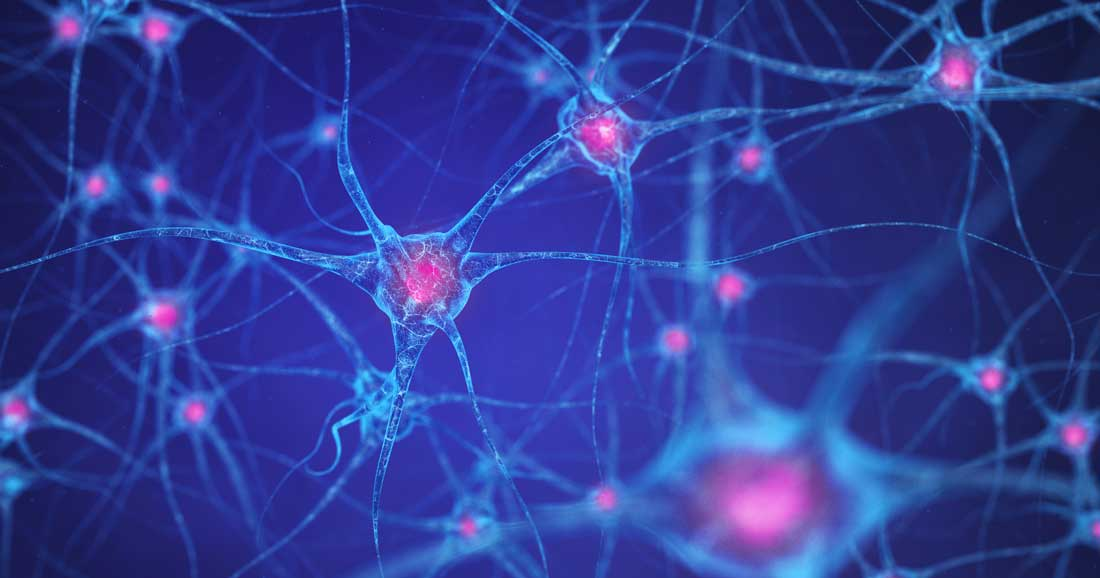
\includegraphics[scale=0.8]{images/image10}
		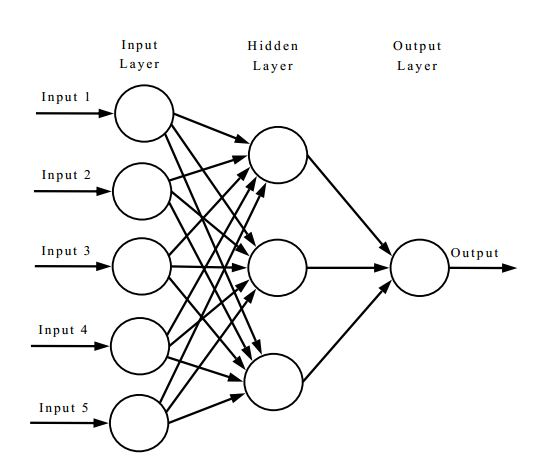
\includegraphics[scale=0.3]{images/image15}
		\caption{Nơ-ron của người (trái) và Mạng nơ-ron (phải)}
	\end{figure}

	Vì thời gian nghiên cứu và lượng dữ liệu thu thập còn hạn chế, phương pháp Transfer Learning được áp dụng. Transfer Learning là phương pháp ứng dụng một mô hình đã được luyện để giải một bài toán vào một bài toán khác có tính chất tương tự. Thông thường, xây dựng một mô hình từ đầu cần một lượng dữ liệu rất lớn, nhưng không phải dữ liệu nào cũng dễ dàng thu thập được. Với hai bài toán tương tự nhau, mô hình giải quyết được bài toán này sẽ không cần quá nhiều dữ liệu để làm quen và giải quyết được bài toán kia. Vì vậy, một mô hình xây dựng từ Transfer Learning sẽ tiết kiệm thời gian tự học, không cần lượng dữ liệu khổng lồ nhưng vẫn cho kết quả khả quan.

	Các mô hình được thử nghiệm trong dự án bao gồm: InceptionV3, MobileNetV2, ResNet50V2, VGG16 và Xception. Những mô hình này đều đã được học qua ImageNet\footnote{Một tập dữ liệu ảnh khổng lồ, phục vụ cho bài toán Phân loại Vật thể.} và được tiếp tục luyện trên toàn bộ mạng bằng dữ liệu mới mà không đóng băng bất cứ thông số nào.

	\begin{table}[H]
		\centering
		\begin{tabular}{|c|c|c|}
		\hline
		Kiến trúc   & Số lượng tham số (triệu) & Số tầng \\ \hline
		InceptionV3 & 24                       & 48      \\
		MobileNetV2 & 2,2                      & 54      \\
		ResNet50V2  & 25                       & 50      \\
		VGG16       & 138                      & 16      \\
		Xception    & 23                       & 71      \\ \hline
		\end{tabular}

		\caption{Thông số của các kiến trúc được thử nghiệm}
	\end{table}

	Các Siêu Tham số (Hyperparameter)\footnote{Các tham số mà mô hình không thể tự học, phải được điều chỉnh thủ công.} được sử dụng cho các mô hình bao gồm:

	\begin{itemize}
		\item Batch size: 24
		\item Epochs: 50
		\item Hàm mất mát: Categorical Cross-Entropy
		\item Hàm tối ưu: Stochastic Gradient Descent ($\alpha$ = 0.001, $\eta$ = 0.9)
		\item Hàm tiêu biến: L2 Regularization ($\lambda = 5 \times 10^{-4}$)
	\end{itemize}

	\null

	Hàm mất mát: \textbf{Categorical Cross-Entropy}, thường được áp dụng vào các bài toán phân loại, vector của giá trị thực sẽ có dạng One-hot Encoding và giá trị đầu vào là kết quả của hàm Softmax/Sigmoid.

	Hàm tối ưu: \textbf{Stochastic Gradient Descent}, mỗi bước duyệt chỉ tính đạo hàm của hàm mất mát trên một điểm dữ liệu $x_i$, rồi lập tức cập nhật các trọng số $w$ ở các tầng. Mặc dù đơn giản nhưng hàm này trên thực tế lại cho kết quả tốt hơn RMSProp hay Adam, vốn phức tạp hơn nhiều.

	Hàm tiêu biến: \textbf{L2 Regularization}, giúp mạng nơ-ron tránh được overfitting bằng cách đưa các tham số về giá trị gần bằng 0 với hàm norm-2, giảm độ phức tạp của mô hình.

	Các mô hình được huấn luyện trên môi trường Google Colab (GPU NVIDIA Tesla K80). Thư viện Keras được sử dụng để xây dựng và huấn luyện cho mô hình.

	\begin{figure}[H]
		\centering
		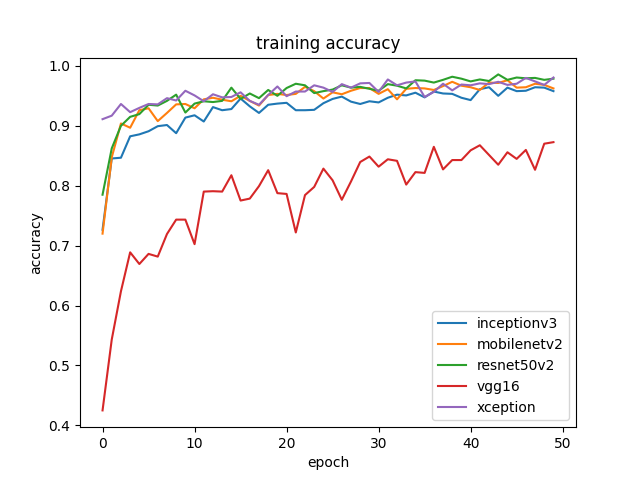
\includegraphics[scale=0.45]{images/accuracy.png}
		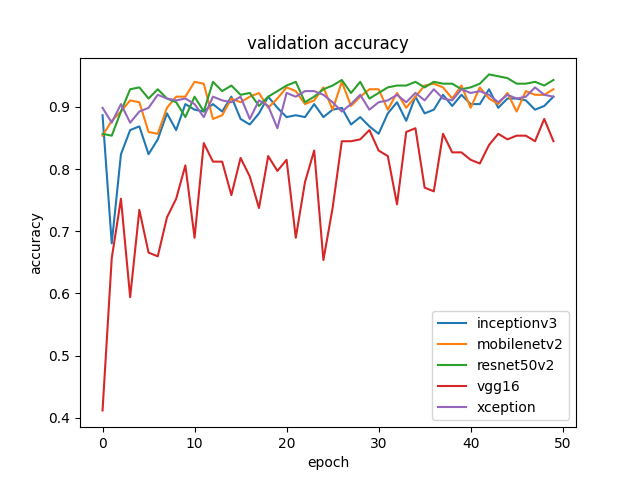
\includegraphics[scale=0.45]{images/val_accuracy.png}
		\caption{Biểu đồ accuracy trên training set và validation set}
	\end{figure}

	\begin{figure}[H]
		\centering
		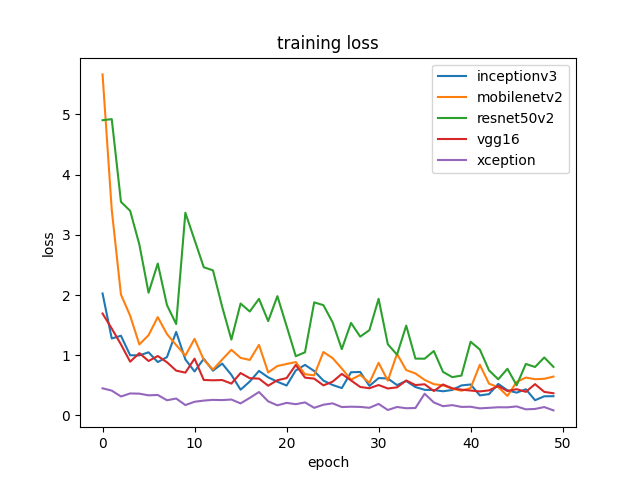
\includegraphics[scale=0.45]{images/loss.png}
		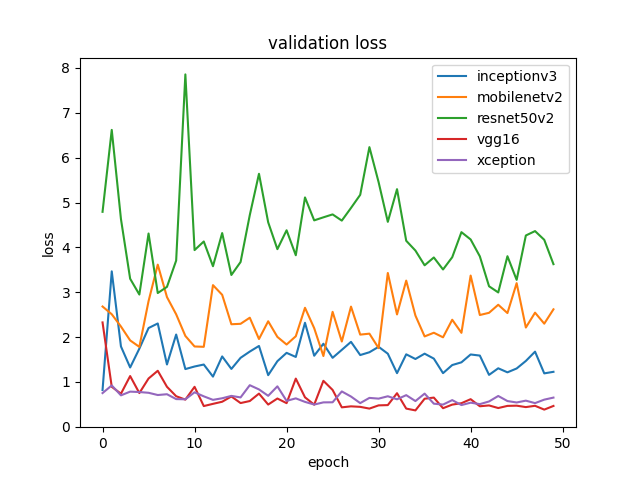
\includegraphics[scale=0.45]{images/val_loss.png}
		\caption{Biểu đồ loss trên training set và validation set}
	\end{figure}
	
	\begin{table}[H]
		\centering
		\begin{tabular}{|c|c|c|c|}
			\hline
			Kiến trúc   & Accuracy (\%) & Precision (\%) & Recall (\%) \\ \hline
			InceptionV3 & \textbf{93}   & \textbf{93}    & \textbf{93} \\
			MobileNetV2 & 90            & 90             & 90          \\
			ResNet50v2  & \textbf{93}   & \textbf{93}    & \textbf{93} \\
			VGG16       & 84            & 84             & 84          \\
			Xception    & \textbf{93}   & \textbf{93}    & \textbf{93} \\ \hline
		\end{tabular}
		\caption{Kết quả đo các mô hình trên test set}
	\end{table}

	Ba mô hình InceptionV3, ResNet50V2 và Xception đều có kết quả đo tương đương: 93\% trên cả Accuracy, Precision và Recall, vượt trội so với MobileNetV2 và VGG16.
	
	Dựa trên các biểu đồ khi huấn luyện, Xception có tốc độ học nhanh và chính xác, InceptionV3 không thua kém quá nhiều, còn ResNet50V2 không ổn định trong suốt quá trình học.

	\begin{figure}[H]
		\centering
		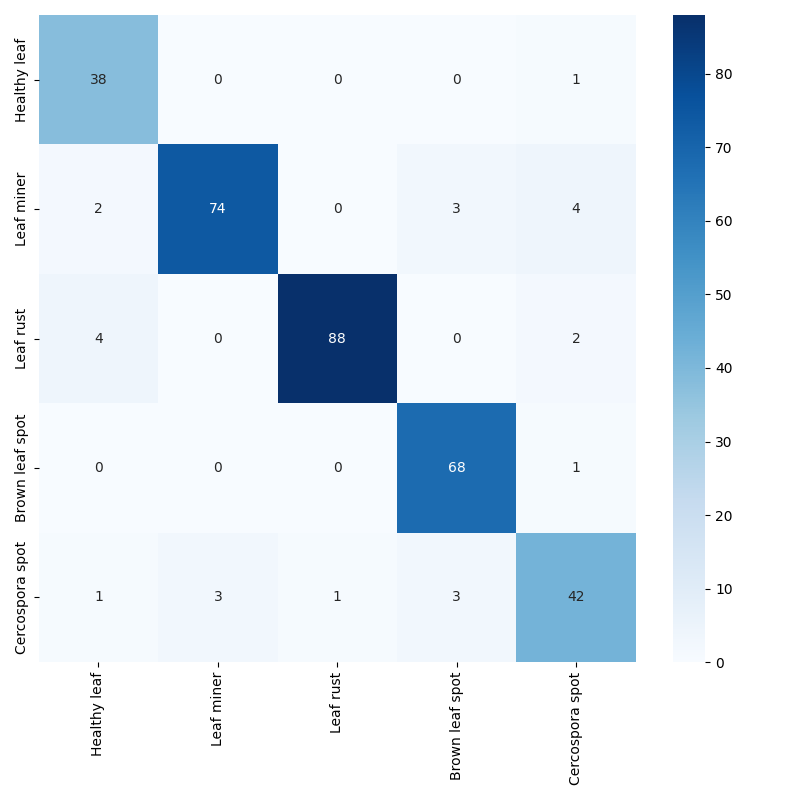
\includegraphics[scale=0.5]{images/xception_matrix.png}
		\caption{Confusion Matrix của Xception}
	\end{figure}

	Sau quá trình nghiên cứu và thử nghiệm, mô hình \textbf{Xception} là mô hình phù hợp nhất với bài toán. Mô hình này là một Mạng Nơ-ron Tích chập (Convolutional Neural Network), thường được sử dụng cho các bài toán phân loại, với ưu điểm là gọn nhẹ, tính toán nhanh mà vẫn đảm bảo độ chính xác.

	"Xception" nghĩa là "Extreme Inception", vì cấu trúc của mô hình này được dựa trên mô hình Inception, nhưng lại mạnh mẽ hơn.

	\begin{figure}[H]
		\centering
		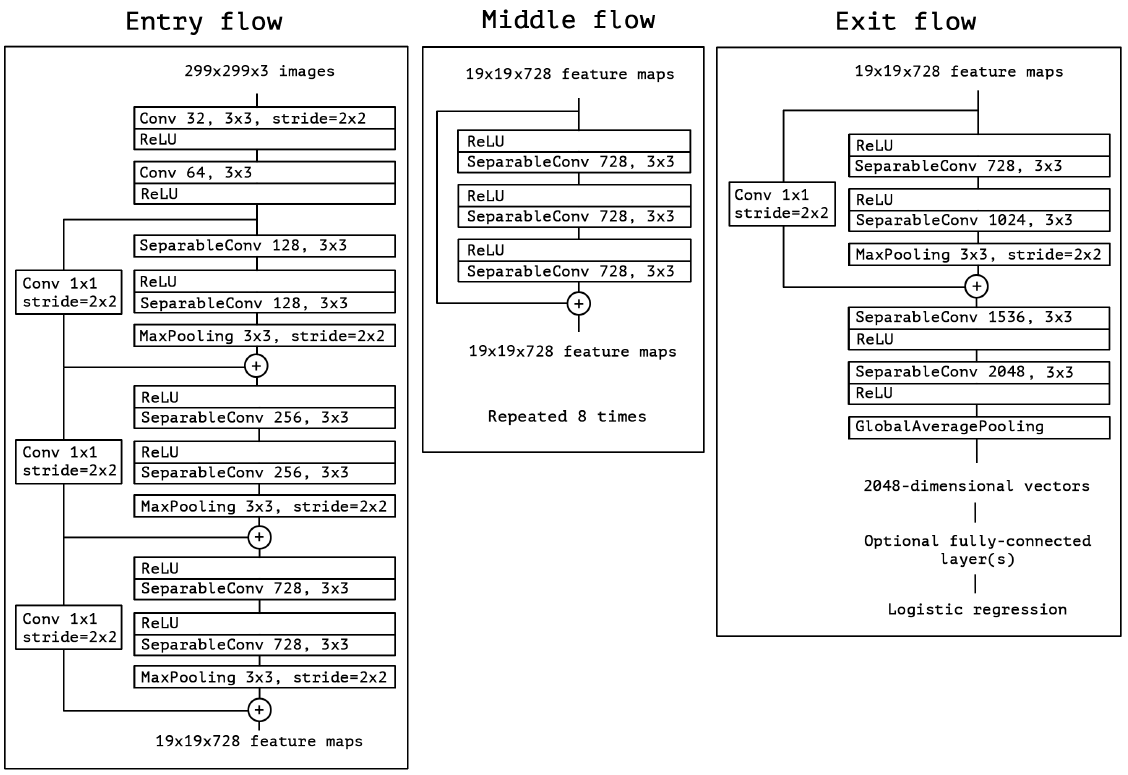
\includegraphics[scale=1]{images/xception_model_doc.png}
		\caption{Mô hình Xception}
	\end{figure}

	\pagebreak

	Xception thừa hưởng các đặc điểm của Inception: 
	
	\begin{itemize}
		\item  Giải quyết được vấn đề representational bottlenecks (thắt cổ chai): kích thước của các tầng không bị giảm một cách đột ngột.
		\item  Thay vì phải chọn một kích thước cố định cho convolution kernel, mô hình được tự chọn kernel thích hợp trong quá trình huấn luyện.
	\end{itemize}

	\null

	Trong mô hình Inception, đầu vào ban đầu được nén bằng phép tích chập 1x1. Với mỗi không gian đầu vào, các bộ lọc khác nhau được áp dụng trên mỗi không gian chiều sâu. Mô hình Xception đảo ngược lại phương pháp này: áp dụng các bộ lọc trước, rồi mới nén không gian đầu vào bằng phép tích chập 1x1 khắp chiều sâu của mô-đun. Phương pháp này gần như giống hệt phương pháp Tích chập chiều sâu tách biệt (áp dụng một bộ lọc trên một kênh đơn lẻ).

	\begin{figure}[H]
		\centering
		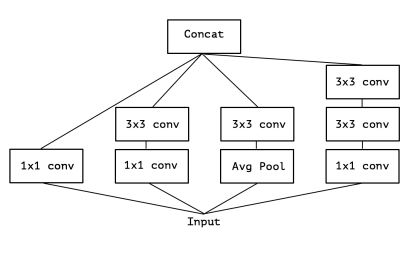
\includegraphics[scale=0.7]{images/inceptionv3.png}
		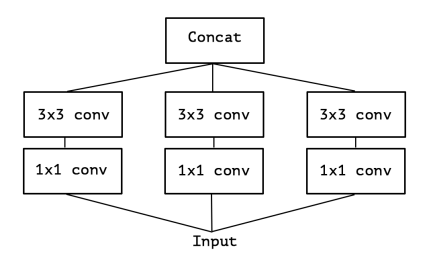
\includegraphics[scale=0.7]{images/simplified_inceptionv3.png}
		\caption{Mô-đun của InceptionV3 (trái) và phiên bản lược giản (phải)}
	\end{figure}

	\begin{figure}[H]
		\centering
		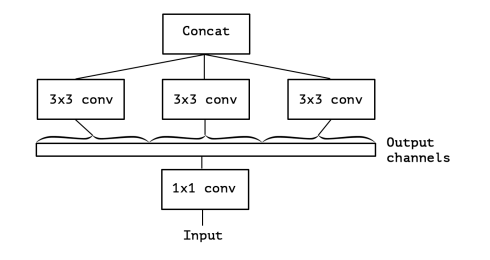
\includegraphics[scale=0.63]{images/strict_equivalent.png}
		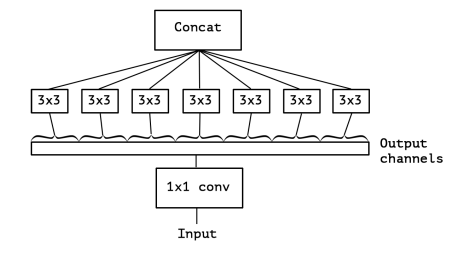
\includegraphics[scale=0.63]{images/xception.png}
		\caption{Mô-đun của Xception (trái) và phiên bản hoàn thiện (phải)}
	\end{figure}

	\begin{figure}[H]
		\centering
		\captionsetup{justification=centering}
		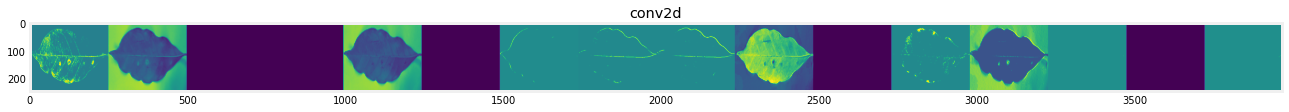
\includegraphics[scale=0.32]{images/image5}
		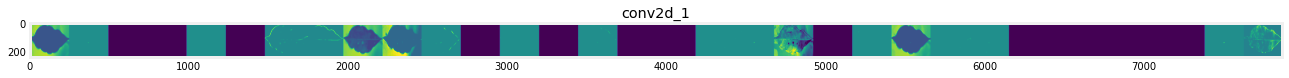
\includegraphics[scale=0.32]{images/image6}
		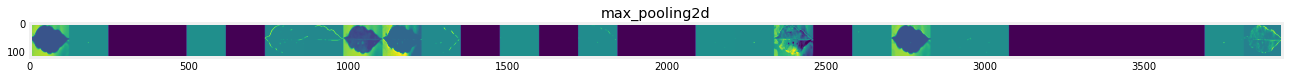
\includegraphics[scale=0.32]{images/image4}
		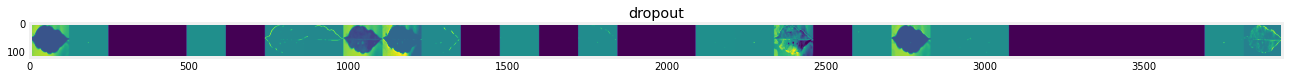
\includegraphics[scale=0.32]{images/image8}
		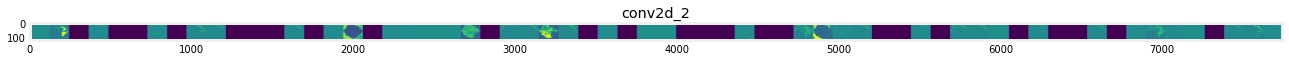
\includegraphics[scale=0.32]{images/image12}
		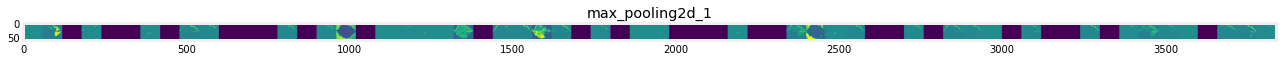
\includegraphics[scale=0.32]{images/image14}
		\caption{Kết quả xử lý của các nơ-ron của một vài tầng\\(đối chiếu với Hình 4)}
	\end{figure}

	\subsection{Ứng dụng Di động}
	Để ứng dụng kết quả từ mô hình trên vào thực tế, tác giả đã phát triển một ứng dụng di động, liên lạc với máy chủ để xử lý.

	\begin{figure}[H]
		\centering
		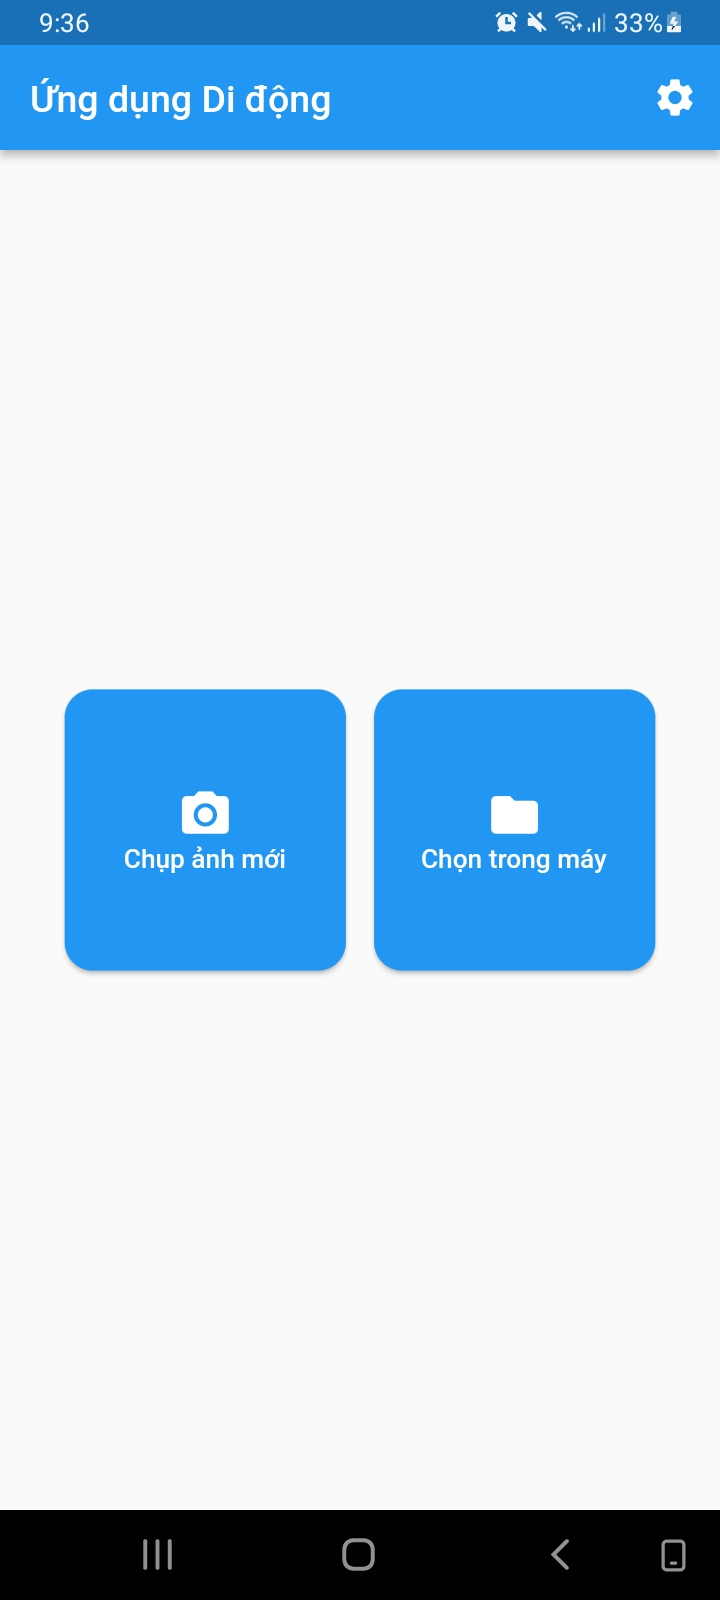
\includegraphics[scale=0.1]{images/screenshot1.jpg}
		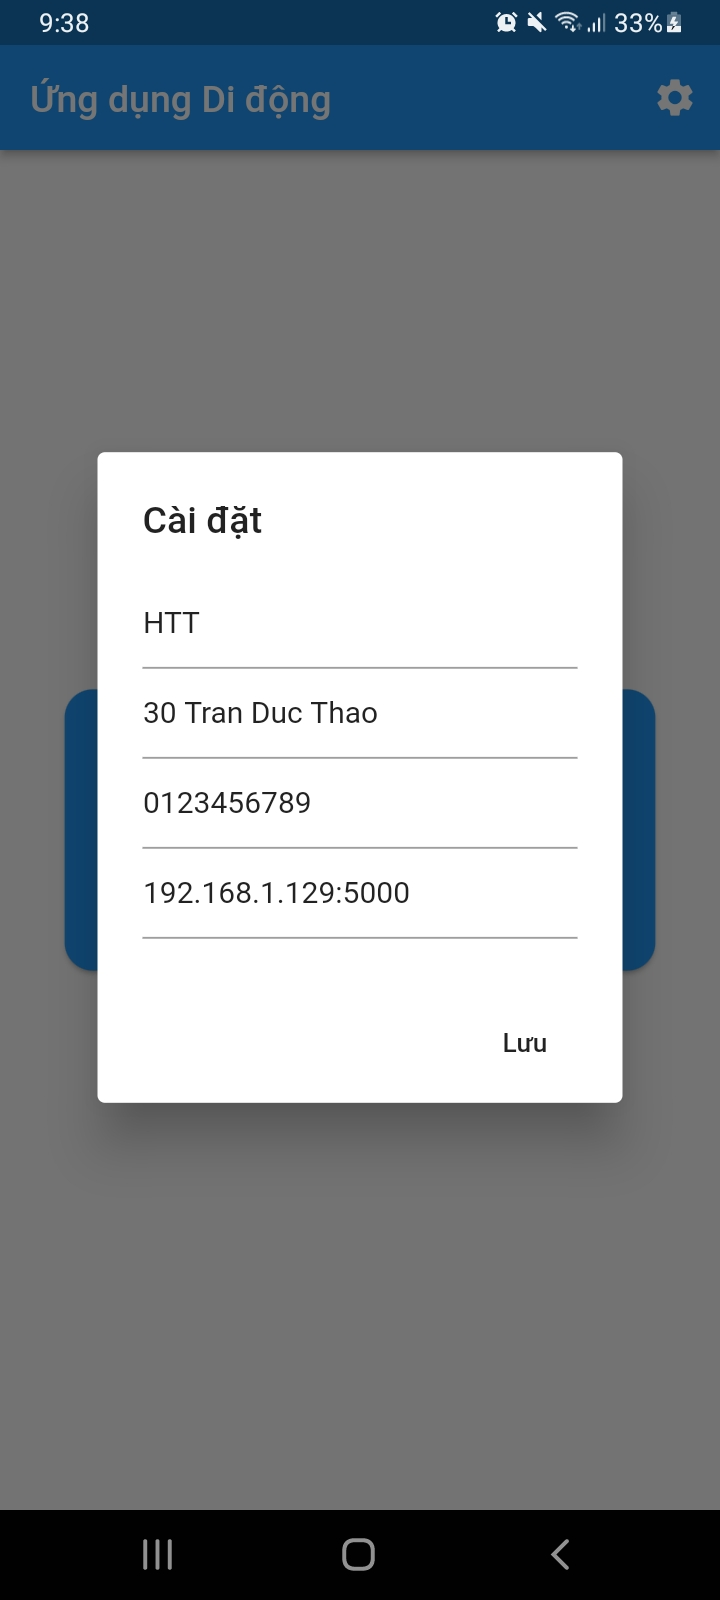
\includegraphics[scale=0.1]{images/screenshot2.jpg}
		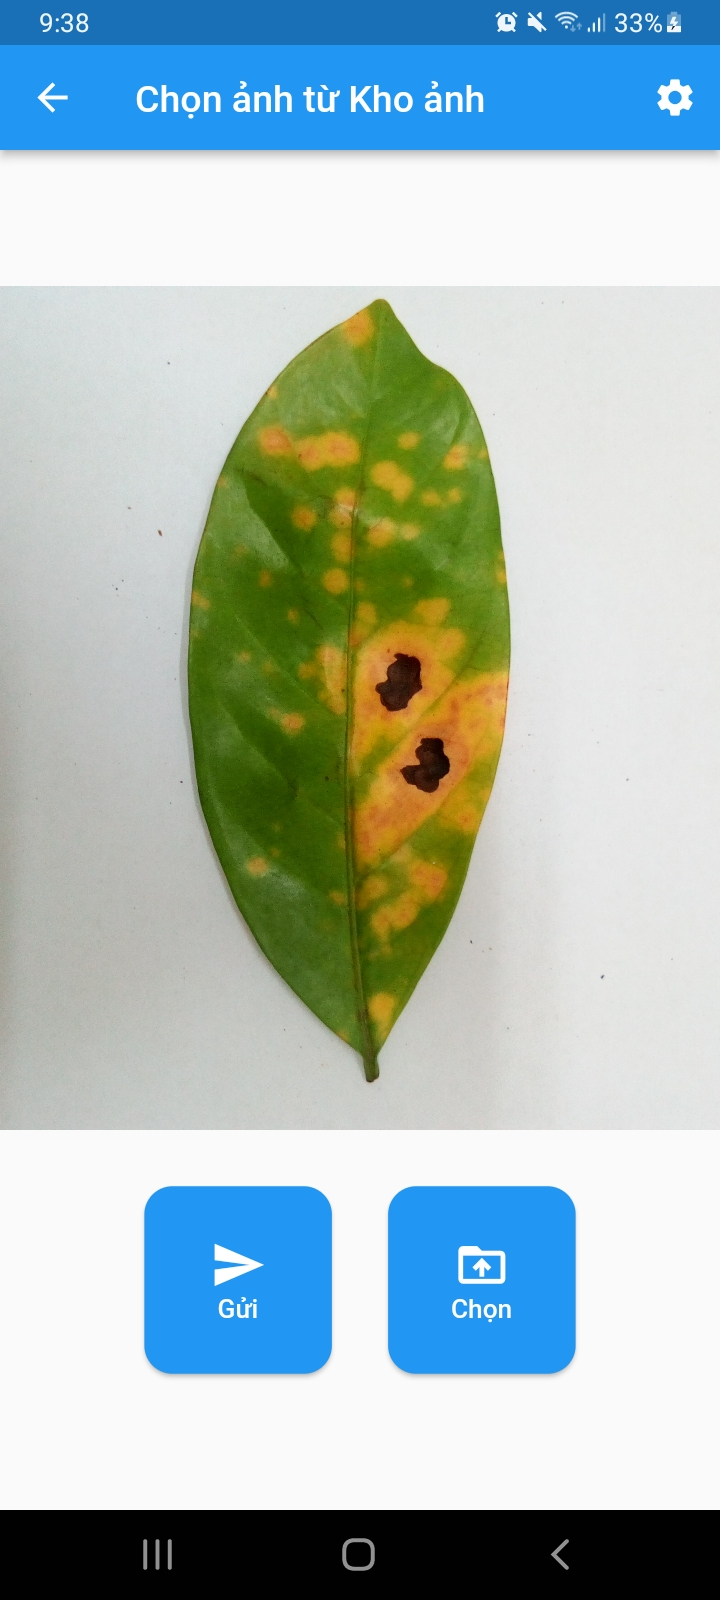
\includegraphics[scale=0.1]{images/screenshot3.jpg}
		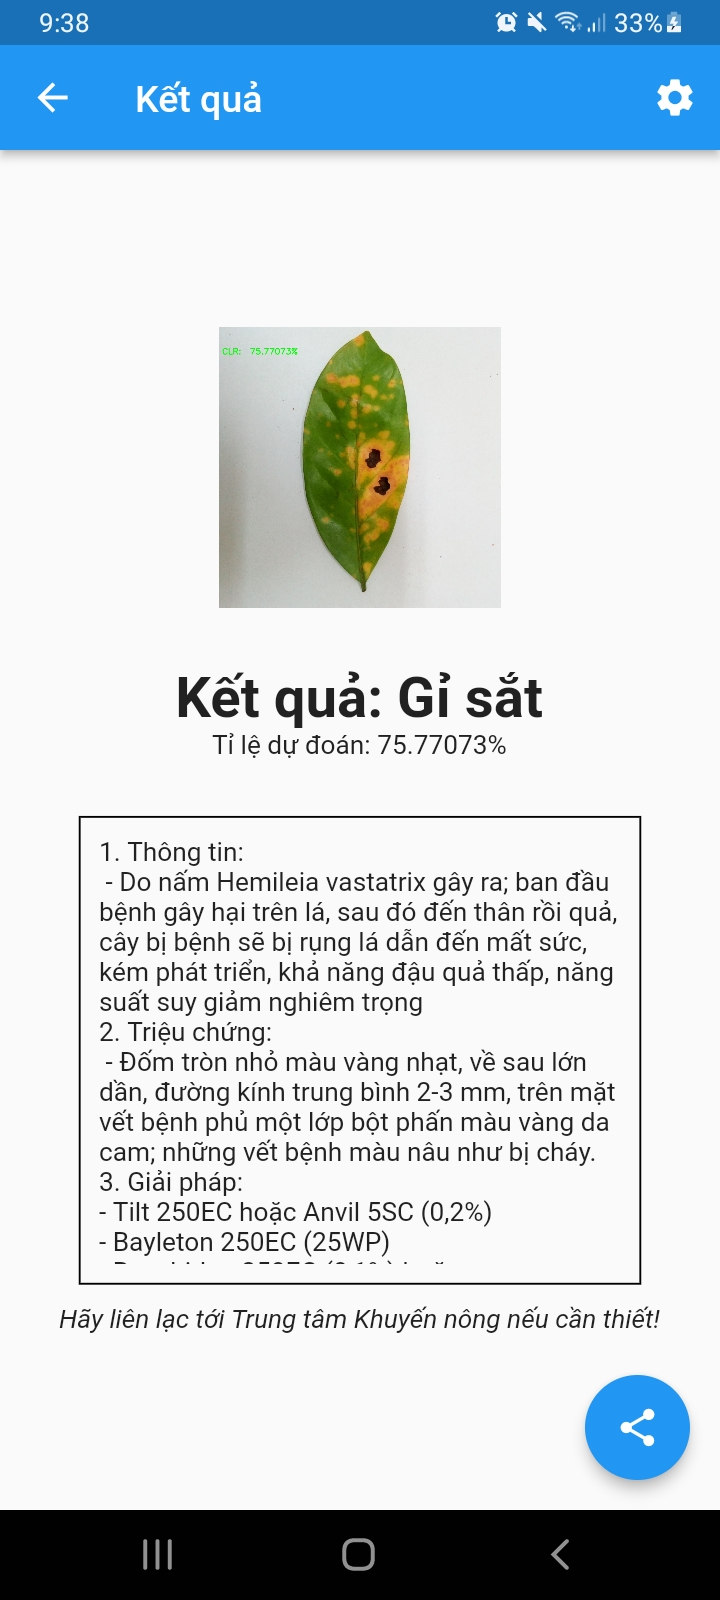
\includegraphics[scale=0.1]{images/screenshot4.jpg}
		\caption{Giao diện của ứng dụng di động}
	\end{figure}

	Ứng dụng được thiết kế đơn giản, gọn nhẹ, dễ sử dụng với bà con, đặc biệt là đồng bào dân tộc thiểu số.

	Ứng dụng cho phép người dùng gửi hình ảnh (ảnh có sẵn trong máy hoặc ảnh chụp mới) lên máy chủ. Máy chủ tiếp nhận ảnh, xử lý ảnh bằng mô hình được xây dựng, rồi trả kết quả chẩn đoán về lại ứng dụng. Các kết quả trả về bao gồm tên bệnh, một số triệu chứng, đặc điểm đặc trưng và tên một vài thuốc đặc trị cho sâu bệnh.

	Ứng dụng được xây dựng bằng framework Flutter, trên ngôn ngữ Dart. Điểm mạnh của Flutter là dễ học, tường minh, hiệu năng tốt, được sử dụng để phát triển ứng dụng đa nền tảng (hoạt động trên cả Android lẫn iOS). Tuy khá mới, nhưng Flutter lại rất được ưa chuộng trong giới phát triển ứng dụng di động hiện nay, được Google hỗ trợ và các công ty lớn khác sử dụng.

	\begin{figure}[H]
		\centering
		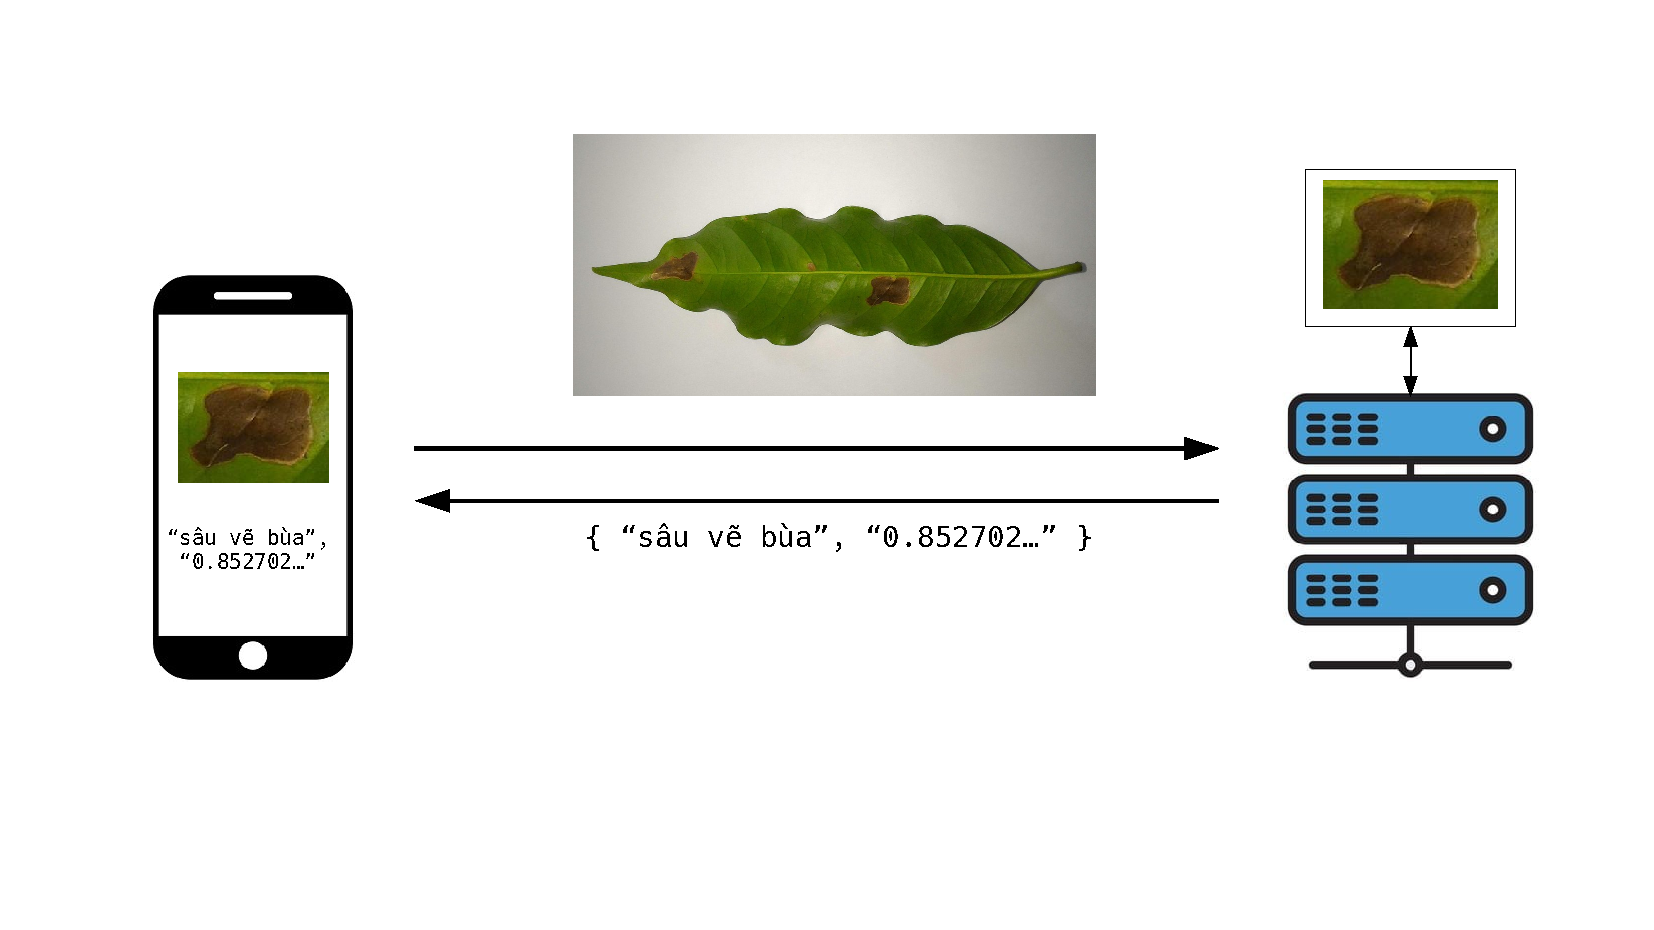
\includegraphics[scale=0.4]{images/chart.pdf}
		\caption{Sơ đồ hoạt động}
	\end{figure}

		
\section{Đánh giá chung}
	Đề tài này nghiên cứu việc ứng dụng Trí tuệ Nhân tạo vào việc nhận diện một số sâu bệnh thường gặp, thông qua biểu hiện của lá. Dữ liệu cho việc rèn luyện được thu thập từ khu vực bản địa của tác giả, song song với tìm kiếm trên mạng [4]. Một số Mạng Tích chập đã được thử nghiệm, trong đó Xception mang lại kết quả tốt nhất. Để ứng dụng mô hình vào thực tế, một ứng dụng di động đơn giản đã được xây dựng, có chức năng gửi và tiếp nhận thông tin từ mô hình.
	
	Trí tuệ Nhân tạo là một phương pháp khả thi để nhận diện sâu bệnh qua hình thái của lá cà phê, và hoàn toàn có thể tiếp tục phát triển trong tương lai, mở rộng sang nhiều giống cây trồng khác, phục vụ người nông dân ở khắp mọi miền đất nước.

	\subsection{Ưu điểm}
	\begin{itemize}
		\item Tỉ lệ nhận diện mang lại hiệu quả tương đối chính xác;
		\item Tiết kiệm thời gian, công sức, chi phí cho việc chẩn đoán so với các phương pháp hiện có;
		\item Ứng dụng di động gọn nhẹ, đơn giản, dễ sử dụng.
	\end{itemize}

	\subsection{Nhược điểm}
	\begin{itemize}
		\item Mô hình vẫn chưa thực sự tối ưu, quá trình rèn luyện chưa đạt kết quả tốt nhất, tốc độ nhận diện còn chậm;
		\item Kích thước tập dữ liệu để rèn luyện còn hạn chế, cần được mở rộng và làm phong phú thêm;
		\item Cần bổ sung thêm cơ sở dữ liệu về sâu bệnh và các thông tin liên quan.
	\end{itemize}

	\subsection{Hướng phát triển}
	\begin{itemize}
		\item Cải tiến mô hình, cải tiến phương pháp luyện để khai thác hết tiềm năng của mô hình, thử nghiệm với những mô hình mới;
		\item Thu thập thêm dữ liệu, xây dựng một bộ cơ sở dữ liệu trung tâm;
		\item Hoàn thiện, phát triển thêm tính năng cho ứng dụng di động;
		\item Hợp tác với các nhà nghiên cứu về cây cà phê để tiếp tục hoàn thiện dự án.
	\end{itemize}

\section{Kết luận}
Mục đích nghiên cứu của dự án xuất phát từ tình hình thực tiễn tại chính địa phương nơi tác giả đang học tập và sinh sống; với hy vọng đề tài sẽ góp phần cải thiện ngành trồng trọt cà phê ở Kon Tum, giúp người dân, đặc biệt là đồng bào dân tộc thiểu số vươn lên thoát nghèo, làm giàu chính đáng trên quê hương của mình; góp phần phát triển kinh tế của địa phương.

\section{Ghi nhận đóng góp}
Xin gửi lời cảm ơn đặc biệt đến mẹ và em gái của tác giả vì đã luôn ủng hộ, dõi theo và tin tưởng tác giả trên con đường nghiên cứu khoa học.

\null

Xin chân thành cảm ơn:
\begin{itemize}
	\item Thầy Lê Quang Tâm, trường THPT Chuyên Nguyễn Tất Thành, tỉnh Kon Tum
	\item Thạc sĩ Trần Văn Cao Sơn, Sở Nông nghiệp \& Phát triển nông Thôn tỉnh Kon Tum
	\item Anh Bùi Đình Nguyên Khoa, trường Đại học Khoa học Tự nhiên - ĐHQG TP.HCM
	\item Anh Nguyễn Hoàng Khang, trường Đại học Khoa học Tự nhiên - ĐHQG TP.HCM
	\item Anh Hồ Khánh Duy, trường Đại học Khoa học Tự nhiên - ĐHQG TP.HCM
	\item Gia đình ông Mai Văn Khá, Thị trấn Đăk Hà, huyện Đăk Hà, tỉnh Kon Tum
	\item Gia đình ông Nguyễn Đức Vũ, Thị trấn Đăk Hà, huyện Đăk Hà, tỉnh Kon Tum
	\item Gia đình ông Hoàng Nguyên Chiến, xã Ia Chim, thành phố Kon Tum, tỉnh Kon Tum
	\item Chị Phạm Xuân My, trường Đại học Luật TP.HCM
\end{itemize}
	đã hỗ trợ tác giả hoàn thành đề tài nghiên cứu này.

\section{Tài liệu tham khảo}
[1] Suhartono, Derwin \& Aditya, Wahyu \& Lestari, Miranty \& Yasin, Muhammad. (2013). Expert System in Detecting Coffee Plant Diseases. International Journal of Electrical Energy. 156-162. 10.12720/ijoee.1.3.156-162.

[2] M. Kumar, P. Gupta, P. Madhav and Sachin, "Disease Detection in Coffee Plants Using Convolutional Neural Network," 2020 5th International Conference on Communication and Electronics Systems (ICCES), 2020, pp. 755-760, doi: 10.1109/ICCES48766.2020.9138000.

[3] Esgario, J. G., Krohling, R. A., \& Ventura, J. A. (2020) "Deep learning for classification and severity estimation of coffee leaf biotic stress" Computers and Electronics in Agriculture 169, 105162,\\doi:10.1016/j.compag.2019.105162

[4] Krohling, Renato; esgario, José; Ventura, Jose A. (2019), “BRACOL - A Brazilian Arabica Coffee Leaf images dataset to identification and quantification of coffee diseases and pests”, Mendeley Data, V1, doi: 10.17632/yy2k5y8mxg.1

[5] François Chollet, "Xception: Deep Learning with Depthwise Separable Convolutions", arXiv:1610.02357v3 [cs.CV], Apr 2017.

\end{document}
